\documentclass{article}
\usepackage{graphicx}
\usepackage{pgfplots,pgfplotstable}
\pgfplotsset{compat=newest}
\begin{document}
\graphicspath{{images/}}
\section*{Introduction}
We attempt to experimentally determine the speed of sound in air utilising microphones to record Boom Whackers of varying notes, generating FFT graphs, and utilising those graphs to establish their respective first harmonics.

\subsection*{Theory}
The relationship between the wavelength ($\lambda$) and length ($L$) at the $n^{th}$ harmonic is given by
\begin{equation}\label{eq:LambdaLength} \lambda_n = \frac{4}{n}L \end{equation}

In practice the ``acoustic'' length ($L$) of the tube is longer than its physical length ($L_p$), which we must account for with an end-correction given by
\begin{equation}\label{eq:AccousticLength} L = L_p + \frac{\pi}{8}\cdot D \end{equation}

The basic wave equation, which describes the proportionality between frequency and wavelength:
\begin{equation}\label{eq:WaveEquation} c = \lambda f\end{equation}

We also expect the $n^{th}$ harmonic to have frequency $n$ times that of the fundamental frequency
\begin{equation}\label{eq:NthHarmonicFrequency} f_n = n\cdot f_1 \end{equation}

Theoretical speed of sound in air: $ 331,5\sqrt{\frac{T}{273}} = 344,6 ms^{-1}$ \\

\subsection*{Variables}
Dependent: Frequency ($f$) \\
Independent: Length of tubes ($L_p$)\\
Control: Room temperature (Only relevant for comparison with theoretical speed of sound)\\

\section*{Data Collection}
Temperature of the room: 295,0 K \\
Diameter of tubes: 4,30 cm $\pm$ 0,05 cm

\begin{table}[h!]
	\caption{Raw data and initial processing}
	\label{table:RawData}
	\begin{tabular}{| c c c p{2cm} |}
		\hline
		Note  & $ L_p \pm$ 0,1 (cm) & $L \pm 0,2$ (cm) & Fundamental frequency $\pm$ 2 (Hz)\\
		\hline
		Mid C & 64,2 & 65,9 & 130\\
		D     & 57,0 & 58,7 & 147 \\
		E     & 50,6 & 52,3 & 163 \\
		F     & 48,7 & 50,4 & 175 \\
		C     & 32,5 & 34,2 & 265 \\
		\hline
	\end{tabular}
\end{table}

\begin{figure}[h!]
	\caption{FFT for mid C, which demonstrates the points at which we can observe harmonics. Its peaks in amplitude are graphed in figure \protect \ref{gr:MidC_FrequencyByWavelength}.}
	\label {fig:FFTMidC}
	\includegraphics[scale=0.3]{fft.png}
\end{figure}
\pagebreak

\section*{Analysis}
\subsection*{How do we know that it's a quarter wave resonator?}
We look at the largest peak in the FFT ($n_1$), figure \ref{fig:FFTMidC}, which we will call the fundamental frequency ($f_1$), and calculate the wavelength at that point ($\lambda_1$). In order to establish whether this is a quarter wave resonator, the next peak in the FFT ($n_2$) should be the \textbf{third} harmonic, so $f_2 = 3f_1$. The following peak should be $f_3 = 5f_1$ and so on. This can be visualised in the x-axis of the graph, by looking at the spacing between the first peak and each peak, which should increase by a factor of an incrementing odd number. We utilise this information to establish theoretical values (discussed further in the report) and to discard peaks due to interference.

Now we may calculate the wavelength ($\lambda_1$) at the fundamental frequency utilising equation \ref{eq:LambdaLength}, and all the subsequent ones, which we graph in figure \ref{gr:MidC_FrequencyByWavelength}. 
$$\lambda_1 = 4 \cdot 65,9 = 263,6 cm \pm 2 $$

\begin{figure}[h!]
	\caption{Frequency x Wavelength plotting of Mid C's multiple harmonics . Note that each point represents one of the peaks in the FFT graph.}
	\label{gr:MidC_FrequencyByWavelength}
	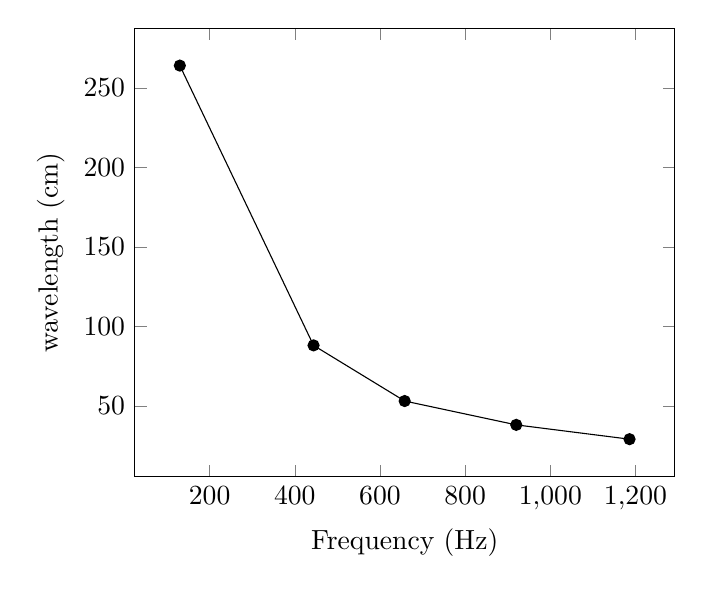
\begin{tikzpicture}
		\begin{axis}[xlabel=Frequency (Hz), ylabel=wavelength (cm)]
			\addplot[color = black, mark = *] coordinates {
				(130,264)(444,88)(658,53)(920,38)(1186,29)
		};
		\end{axis}
	\end{tikzpicture}
\end{figure}

Rearranging equation \ref{eq:WaveEquation}, we arrive at the following equation $\lambda = \frac{c}{f}$, which allows us to plot $\frac{1}{f} \times \lambda$, giving a line such that its slope is the speed of the wave, $c$.

\begin{figure}[h!]
	\caption{Frequency$^{-1}$ x Wavelength plotting of Mid C's multiple harmonics.}
	\label{gr:MidC_1/FrequencyByWavelength}
	\begin{tikzpicture}
		\begin{axis}[xlabel=Frequency$^{-1}$ (s), ylabel=wavelength (m)]
			\addplot+ [only marks, forget plot,error bars/.cd,y dir=both,y explicit relative,
			x dir=both, x explicit relative]
				table[x=x, y=y, y error = ey, x error = ex] {FrequencyPlot.dat};
			\addplot [mark = none]coordinates {(0,0)(0.0077,2.64)};
			\node[anchor=south] at (axis cs:0.0015,2.45){\footnotesize slope = $340,2 \pm 7,5 $ m/s};
			\node[anchor=south] at (axis cs:0.0015,2.3){\footnotesize y-intercept = $0,03 \pm 0,03$};
			\node[anchor=south] at (axis cs:0.0015,2.15){\footnotesize Correlation = 0,9993};
			\draw[dotted] (0.0010,2.3) -- (0.0034,1.32);
		\end{axis}
	\end{tikzpicture}
\end{figure}
It is clear from the y intercept on figure \ref{gr:MidC_1/FrequencyByWavelength} that we have a systematic error of $0,03 \pm 0,03$. It is also interesting to note that the uncertainty in the wavelength comes from the measurement of the length of the tube, and can't actually be seen in the graph due to being too small. Furthermore, the uncertainty in the frequency was doubled to 2 Hz in order to account for the multiple peaks around a ``main'' peak we observe in figure \ref{fig:FFTMidC}.

\pagebreak
\section*{Conclusion}
The research question was an investigation of the speed of sound, which we have found to be $340,2 \pm 7,5 ms^{-1}$, well within the expected $344,6 ms^{-1}$ theoretical value. There are other interesting things to observe from the experiment, including a comparison between the theoretical and practical frequencies of each harmonic, as described in table \ref{table:TheoreticalXPractical}. There is a fair degree of confidence in the results of our experiment, however, as will be discussed in the Evaluation section, the amount of data is somewhat lacking.
\begin{table}[h!]
	\caption{Comparison of theoretical frequencies ($f_{th}$) and practical ($f_{th}$) for the $n^{th}$ harmonic}
	\label{table:TheoreticalXPractical}
	\begin{tabular}{|c c c c|}
		\hline
		Harmonic & $f_{th}$ (Hz) & $f_{pr}$ (Hz) & \% of Theoretical \\
		\hline
		1 & 130 & 130 & baseline\\
		3 & 390 & 444 & 87,8\%\\
		5 & 650 & 658 & 98,7\\
		7 & 910 & 920 & 98,9\\
		9 & 1170 & 1186 & 98,7\\
		\hline
	\end{tabular}
\end{table}


\section*{Evaluation}
The value of 340,2 m/s found for the speed of sound is just above 1\% off from the theoretical value, which is surprisingly accurate, considering the way the data was analysed, and that it effectively does not involve any repetitions. however for all intents and purposes the uncertainty in the experiment as a whole is almost negligible. The largest issue in the assessment of the experiment was two-fold: It was fairly difficult to get a ``clean'' recording that we could analyse without background noise, or other sorts of interference; and judging what should be counted as a harmonic. The solution to the latter was comparing all peaks in the FFT to theoretical values and discarding the rest \textendash\ the assumption being that the other smaller peaks in the graph are just interference.

After concluding the paper, I noticed the calculations should have been done for the fundamental frequency of all tube lengths, rather than through the analysis of the FFT for one note. The issue with my methodology is, of course, that it does not account for random error, as I'm utilising a non-repeated set of data in order to do all the calculations. The expectation was that the multiple measurements would not necessarily be more accurate, but would provide a better set of data for analysis of errors. My speculation is that it is due to a mixture of both random error in properly doing the experiment, but most importantly the frequency of data collection from the software. When carrying out the experiment, we opted for 1000 data points per second with the other notes, but 10.000 for Mid C, which I utilised in the data analysis.

\begin{figure}[h!]
	\caption{Frequency$^{-1}$ x Wavelength for all tube lengths}
	\label{gr:}
	\begin{tikzpicture}
		\begin{axis}[xlabel=Frequency$^{-1}$ (s), ylabel=wavelength (m)]
		\addplot+ [only marks, forget plot,error bars/.cd,y dir=both,y explicit relative,
		x dir=both, x explicit relative]
		table[x=x, y=y, y error = ey, x error = ex] {varyingLengths.dat};
		\addplot [mark = none]coordinates {(0,0)(0.0077,2.64)};
		\node[anchor=south] at (axis cs:0.0010,2.3){\footnotesize slope = 335,8 m/s};
		\draw[dotted] (0.0010,2.3) -- (0.0034,1.32);
		\end{axis}
	\end{tikzpicture}
\end{figure}


\end{document}
